\documentclass[a4paper,11pt]{article}

\usepackage{graphicx}
\author{Oliver S Burren}
\title{First Year Report}
\begin{document}
\begin{figure}[h]
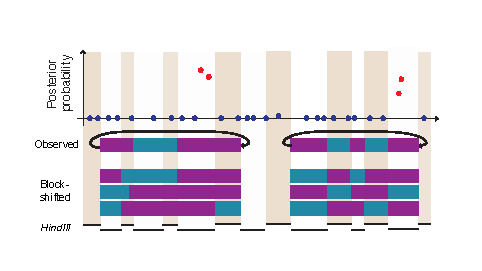
\includegraphics[width=\textwidth]{./figures/blockshifter.pdf}
%\caption{Illustration of circularised permutation strategy employed by \textit{blockshifter} for 'mixed superblocks'. \textit{Hind}III fragments (vertical shading) are assigned to 'superblocks'; these are runs of PIRs for test (purple) and control (turquoise) tissues separated by two or more non PIR fragments (grey). To allow for inflation in test statistics dues to LD in PPI and PIR correlation we  circularise and rotate assignment of blocks to generate permuted superblocks as illustrated, whilst maintaining PIR structure. PPI are then assigned to these permuted superblocks to generate an empirical null distribution of the test statistic.}
\caption{Illustration  of  circularised  permutation  strategy  employed  by blockshifter for  'mixed superblocks'. \textit{Hind}III fragments (vertical  shading) are assigned to 'superblocks';  these are runs of PIRs for test (purple) and control  (turquoise) tissues  separated  by  two or more  fragments that did not interact with any promoter (grey).  PIRs identified in both tissues cannot contribute to any comparative test, but do contribute to the definition of the superblock, and are shown in white.  To allow for correlation in SNP association statistics due to LD and PIR correlation we circularise and rotate assignment of blocks to test or control to generate permuted superblocks as illustrated, whilst maintaining PIR structure.  A blockshifter test statistic compares the average value of the SNP association statistics in test and control blocks, and its null distribution can be calculated by applying the same test with assignments sampled from the permuted data.  While there are a limited number of possible permuted assignments in any one superblock, we aggregate over multiple blocks, allowing fast computation of a null distribution for the blockshifter test statistic.}
\end{figure}
\end{document}
